\section{Java}
Java es un lenguaje de propósito general desarrollado por Sun Microsystems (después adquirida por Oracle) que reúne las siguientes características:
\begin{itemize}
 \item Compilado
 \item Orientado a objetos
 \item Basado en clases
 \item Concurrente 
\end{itemize}

Una de las características que no se mencionó en el listado anterior, pero que son esenciales para entender por qué java ha disfrutado de una enorme popularidad en la escena del desarrollo de software es la capacidad de ejecutar programas en cualquier ambiente que pueda ejecutar la Virtual Java Machine, para describir mejor el proceso, a continuación se presenta una descripción de la arquitectura de un programa en Java:
\begin{figure}[H]
  \begin{center}
    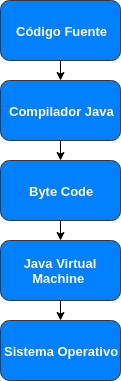
\includegraphics{JavaArch}
  \end{center}
  \caption{Arquitectura del lenguaje Java}
\end{figure}

Como se puede observar en el diagrama anterior, el proceso parte del código fuente del programa, este para por el compilador de Java, generando un ByteCode (archivo .class) el cual será la entrada de la Java Vitual Machine, esta se encargará de transformar el ByteCode a código máquina para su ejecución.

Existen JVM especificas a cada plataforma, es por esto que el mismo programa Java puede ejecutarse en múltiples ambientes y plataformas.


\section{Java EE}
Java EE (Enterprise Edition) es una plataforma para el desarrollo de aplicaciones web a nivel empresarial, proporciona una serie de herramientas que facilitan el desarrollo.
Utiliza el lenguaje de programación Java; provee API's para mapear objetos de alguna base de datos, implementar arquitecturas distribuidas y multicapas, y desarrollar servicios web con un enfoque modular.
Java EE enfatiza el principio \textit{"convención sobre configuración"}, lo que permite al desarrollador enfocarse en la construcción de la aplicación mientras la plataforma se encarga de ciertas configuraciones necesarias para ejecutarse.
Java EE incluye los siguientes paquetes que extienden la funcionalidad de un proyecto de Java SE:

\begin{itemize}
  \item javax/servlet
  \item javax/websocket
  \item javax/faces
  \item javax/faces/component
  \item javax/enterprise/inject
  \item javax/enterprise/context
  \item javax/ejb
  \item javax/validation
  \item javax/persistence
  \item javax/transaction
  \item javax/security/auth/message
  \item javax/enterprise/concurrent 
  \item javax/jms
  \item javax/resource
\end{itemize}
Las aplicaciones Java EE generalmente se justan a un modelo por capas como se muestra en el siguiente diagrama:
\begin{figure}[H]
  \begin{center}
    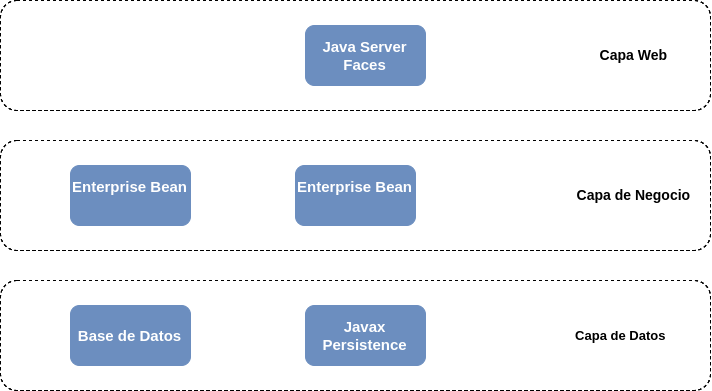
\includegraphics[scale=0.6]{JavaEEArch}
  \end{center}
  \caption{Arquitecturad de una aplicación Java EE}
\end{figure}


\section{Spring}
Spring es un framework para construir aplicaciones compatibles con JVM, esta construido sobre Java EE y proporciona herraminetas para hacer ligero el desarrollo de aplicaciones web.

A continuación se listan algunas de sus características principales: 

\begin{itemize}
  \item Configuración mediante XML 
  \item Manejo de ciclo de vida de componentes
  \item Administración de dependencia entre componentes
  \item Se integra con otros frameworks (JSF, Hibernte, etc.)
  \item Inversión de control
  \item Inyección de dependencias 
\end{itemize}

Spring promueve el desarrollo modular y la separación de aspectos.
Una de las ventajas que ofrece Spring es el poder desarrollar funcionalidades de la aplicación utilizando POJO's (Plain Old Java Object), se utilizan anotaciones para identificar el tipo de objeto y el framework es capaz de unirlos y generar una aplicación completa, a continuación se presenta un ejemplo de un controlador creado bajo el patrón MVC: 

\begin{lstlisting}
  @Controller
  @RequestMapping("/libros")
  public class LibrosController{
  
  	public final InventarioLibros inventario;
  	
  	@RequestMapping(method = RequestMethod.GET)
  	public Map<String> get() {
  	  return inventario.getLibros(); 
  	}
  }
\end{lstlisting}

Cabe resaltar las anotaciones \textit{@Controller} y \textit{@RequestMapping} son proporcionadas por Spring y la lógica es una simple clase de Java, por lo que se agiliza y simplifica el desarrollo.

\section{WildFly}
WildFly es un servidor de aplicaciones de código libre que permite el despliegue de aplicaciones Java.
Es flexible, por lo que se pueden editar diferentes configuraciones dependiendo del proyecto desarrollado.
Entre sus principales características se encuentran:
\begin{itemize}
  \item Soporte para Java EE (última versión de Java EE)
  \item Compatibilidad con tecnologías web modernas, como WebSockets o estándares REST
  \item Soporta paradigmas modulares de aplicaciones Java
\end{itemize} 

\section{Java Server Faces}
JSF es un framework MVC para desarrollar interfaces gráficas en aplicaciones Java EE.
JSF utiliza componentes definidos en archivos xHTML en forma de Facelets.
En general una interfaz construida con JSF está integrada por:
\begin{itemize}
  \item Vista: Facelets
  \item Modelo: Objetos Java
  \item Controlador: ManagedBeans
\end{itemize} 

Entre las ventajas de desarrollar interfaces gráficas con JSF sobre escribir código JavaScript se encuentran:

\begin{itemize}
  \item Acceder a objetos de lógica de negocio fácilmente 
  \item Ofrece un desarrollo seguro y robusto
  \item Fácil de probar y mantener 
\end{itemize}

La API de JSF incluye los siguientes elementos: 
\begin{itemize}
  \item Herramientas para representar componentes de interfaz gráfica y administrar su estado.
  \item Validación.
  \item Navegación.
  \item Manejo de Eventos de cliente y servidor.
  \item Conjunto de componentes por defecto (botones, inputs, etc.).
  \item Beans administrados (Managed beans).
\end{itemize}

\section{PrimeFaces}
PrimeFaces es un framework para construir interfaces gráficas con Java EE.
Es conocido por ser una librería ligera, fácil de usar, centrada en el rendimiento y la simplicidad. Es el framework recomendado en la documentación oficial de Spring para desarrollar frontend con JSF.
Incluye componentes estilizados como inputs, botones, menús, gráficas, además de incluir funcionalidades AJAX.

